\chapter{Dimensionality reduction and clustering}
\label{chap:cluster}
In this chapter, we explore the application of unsupervised learning techniques, specifically dimensionality reduction and clustering, to analyze and interpret high-dimensional CFD simulation data of nozzle flows. Unsupervised learning, a class of machine learning methods that operate on unlabeled data, aims to discover hidden patterns or intrinsic structures within the data. Our objective is to distill high-dimensional simulation data into insightful, low-dimensional representations and identify distinct patterns through clustering, facilitating a deeper understanding of fluid behavior under various conditions. We use \gls{PCA} \cite{pearson1901pca}, and \gls{t-SNE} \cite{tsne} for dimensionality reduction. Subsequently, we apply the \gls{DBSCAN} algorithm \cite{ester1996dbscan} to the reduced-dimensional data to identify distinct clusters representing various fluid flow behaviors.
\section{Dimensionality reduction}
Dimensionality reduction is crucial in simplifying high-dimensional data, making it amenable to visualization and data analysis. Here, we focus on PCA and t-SNE.
\subsection{Principal Component Analysis (PCA)}
PCA is a linear technique that reduces the dimensions of a dataset by transforming them to a new basis, where the axes are the directions of maximum variance. It effectively compresses the data while attempting to retain the original variance in the data.
\subsection{t-Distributed Stochastic Neighbor Embedding (t-SNE)}
t-SNE, a non-linear technique, converts the high-dimensional Euclidean distances between points into conditional probabilities that represent similarities, aiming to preserve the local structure of the data. The cost function minimized by t-SNE is based on the Kullback-Leibler divergence \cite{csis} between the distribution of the high-dimensional data and the distribution of the low-dimensional embedding.
\section{Density-Based Spatial Clustering of Applications with Noise (DBSCAN)}
The DBSCAN algorithm can be employed to identify clusters of varying shapes and sizes based on densities within low-dimensional data, as well as mark outliers in low-density areas. Its idea is to classify points as core points, border points, or outliers, based on the density of their neighborhoods. DBSCAN is defined by a parameter denoting the radius of the neighborhood with respect to a point and another parameter for the minimum number of points required to form a cluster.
\section{Experiments, results and inference}
Dimensionality reduction techniques such as PCA and t-SNE were applied to both transitional and steady-state simulation data constituting the training-validation dataset from surrogate modelling, facilitating the visualization and interpretation of complex flow dynamics. PCA and t-SNE are used to transform the target data to two dimensions, and the results from this transformation can be seen in Figure \ref{pca_sim} and Figure \ref{tsne_sim}. Each data point corresponds to a simulation case and marked by its velocity ratio, which is taken as the ratio of the higher of the two inlet velocities to that of the lower. In the t-SNE plot, we observe clearly distinct clusters of data points on the bottom left and top right corners. The clusters are formed by velocity ratios greater than four, likely indicating the phenomenon of complete adhesion to the Coanda surfaces.\\
Evidenced by the clustering of points with higher velocity ratios, we propose the hypothesis that as the velocity ratio increases, the tendency of the outflow jet to exhibit complete adhesion to one of the surfaces becomes more pronounced. Simulations with lower velocity ratios appear to be more dispersed across the t-SNE plot, which might indicate a more varied flow behavior at these ratios or a weak adhesion effect. The data does not cluster as tightly as those with higher velocity ratios, implying a case of jet deflection without adhesion to surfaces. We also plot the t-SNE data, categorizing each data point based on its inlet velocities relationship as seen in Figure \ref{tsne_in}. The application of DBSCAN to these low-dimensional representations from the t-SNE transformation provides further evidence for our speculated theories with the identification of distinct flow behavior clusters, based on Coanda adhesion phenomena. 
\begin{figure}[ht]
    \centering
    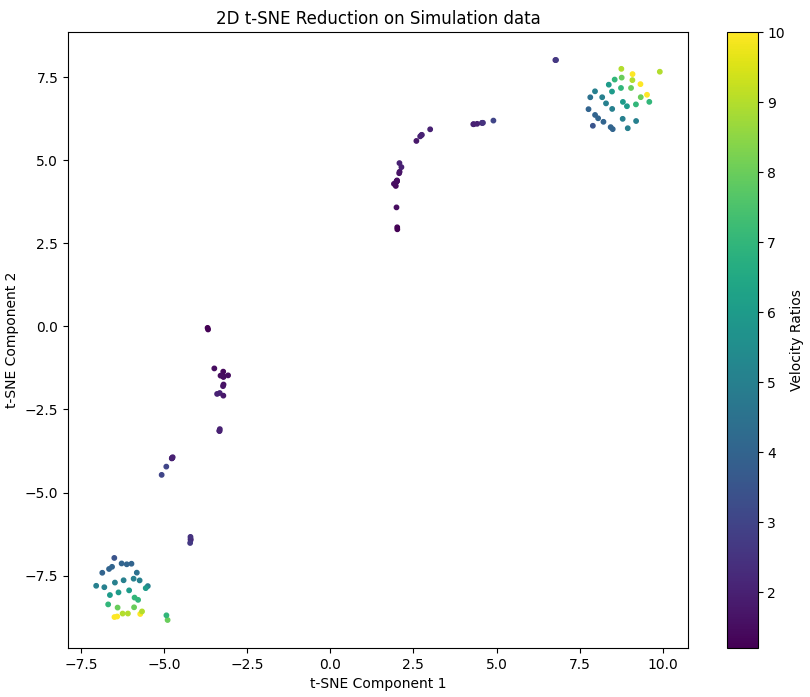
\includegraphics[width=10cm]{images/Clustering/tsne_sim_cmap.png}
    \caption{Scatter plot visualizing the 2D t-SNE reduction of steady-state simulation data, categorized by varying velocity ratios. Each point on the plot represents a simulation data sample, and the color coding corresponds to the velocity ratios.}
    \label{tsne_sim}
    \end{figure}
\begin{figure}[ht]
    \centering
    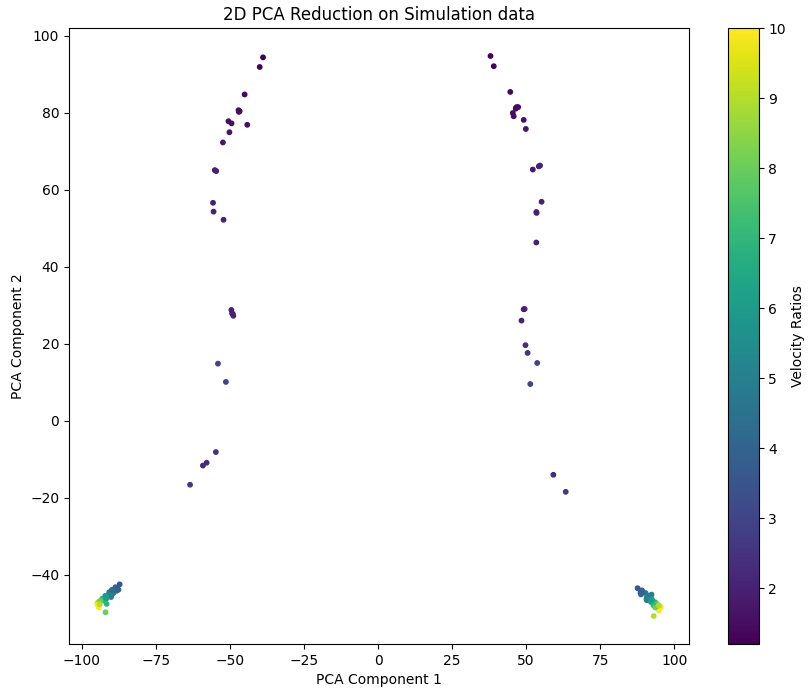
\includegraphics[width=9cm]{images/Clustering/pca_sim_cmap.png}
    \caption{Scatter plot visualizing the 2D PCA reduction of steady-state simulation data, categorized by varying velocity ratios. Each point on the plot represents a simulation data sample, and the color coding corresponds to the velocity ratios. }
    \label{pca_sim}
    \end{figure}
\begin{figure}[ht]
    \centering
    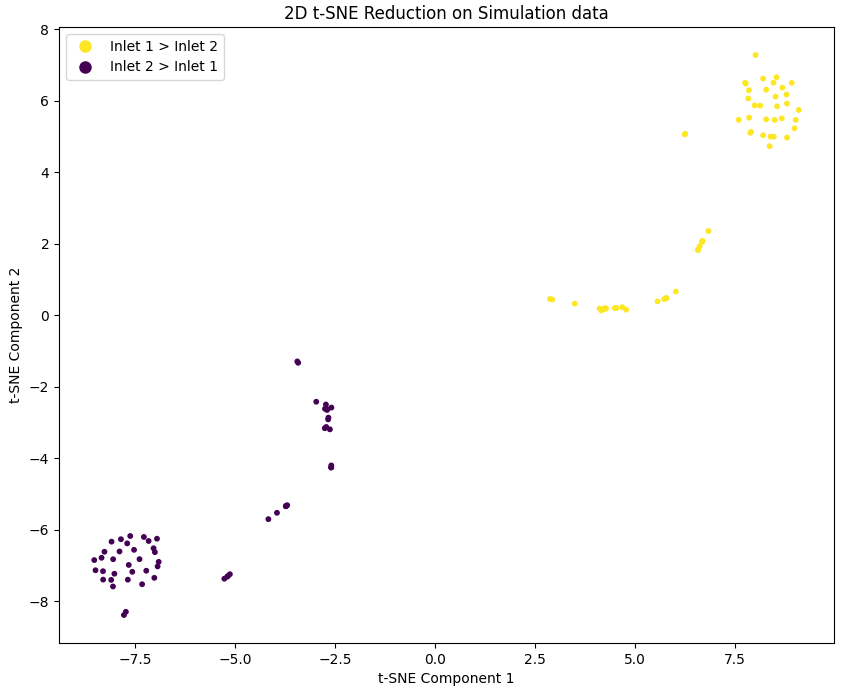
\includegraphics[width=10cm]{images/Clustering/tsne_inlet_cmp.png}
    \caption{Scatter plot visualizing the 2D t-SNE reduction of steady-state simulation data, categorized by Inlet 1 and Inlet 2 relationship.}
    \label{tsne_in}
    \end{figure}
An examination of the scatter plot in Figure \ref{dbscan_tsne} shows two clusters as well as outlier points scarcely distributed between these two regions:
\begin{itemize}
  \item \textbf{Blue cluster (Coanda adhesion to the top surface):} The blue cluster, isolated in the upper quadrant of the plot, likely represents instances of Coanda adhesion to the top surface of the nozzle. The spatial separation of these points from the central mass suggests a specific, consistently observed flow behavior across these simulations.
  \item \textbf{Yellow cluster (Coanda adhesion to the bottom surface):} The cluster circled in yellow, situated in the bottom left of the plot, corresponds to the simulations exhibiting Coanda adhesion to the bottom surface. The compactness and isolated location of this cluster signify a distinct and strong pattern of flow behavior.
  \item \textbf{Purple outlier points (Jet deflection):} The outliers marked in purple, dispersed between the blue and yellow clusters, likely characterize scenarios where the jet deflects towards either surface, representing a transitional behavior that does not culminate in pronounced Coanda adhesion.
\end{itemize}
\begin{figure}[ht]
    \centering
    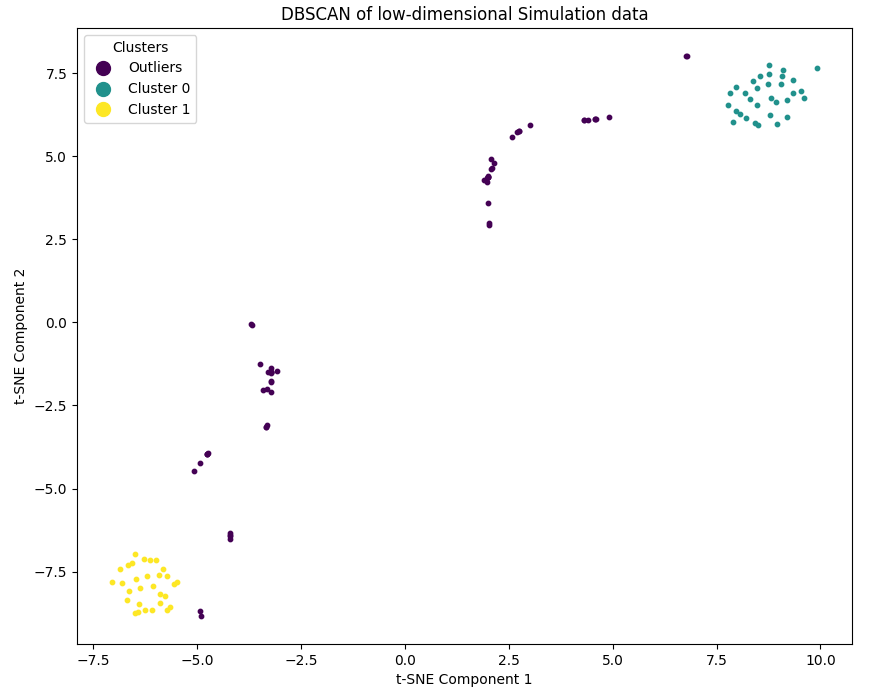
\includegraphics[width=9cm]{images/Clustering/dbscan_tsne_sim.png}
    \caption{DBSCAN clustering visualized on t-SNE-reduced steady-state simulation data.}
    \label{dbscan_tsne}
\end{figure}
We also perform visual inspection of the simulations and classify them into four instances:  
\begin{enumerate}
    \item Complete adhesion to the bottom Coanda surface. 
    \item Jet deflection and partial adhesion to the bottom Coanda surface. 
    \item Complete adhesion to the top Coanda surface. 
    \item Jet deflection and partial adhesion to the top Coanda surface. 
\end{enumerate}
\begin{figure}[ht]
    \centering
    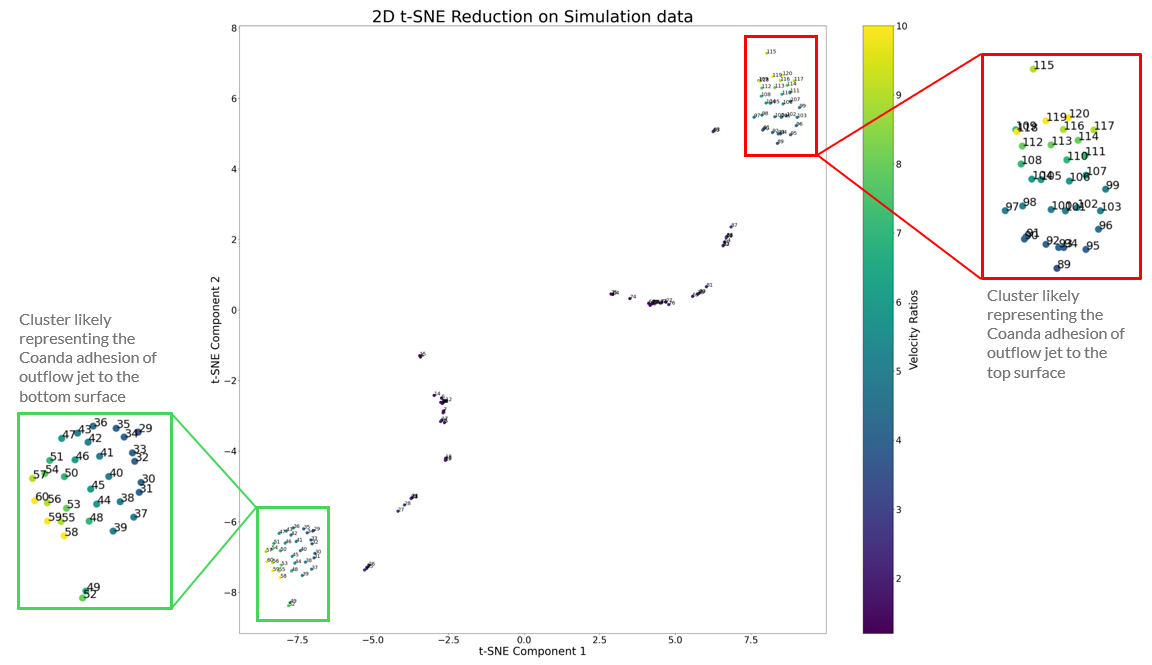
\includegraphics[width=14cm]{images/Clustering/redgreen.png}
    \caption{Annotation of each sample point based on its simulation case. Here, the green box captures the cluster that is representative of cases exhibiting complete Coanda adhesion to the top surface, whereas the red box likely shows the cluster comprising the cases marked by complete Coanda adhesion to the bottom wall. Note that the original clusters are zoomed in for readability.}
    \label{anno}
    \end{figure}
It is observed that the cluster on the bottom left corresponds to cases displaying complete adhesion to the bottom Coanda surface whereas the one on the top right are constituted by cases that show complete Coanda adhesion to the top wall. The classification of the cases is presented in the Appendix \ref{appendix} serve as the ground truth: cases 89 to 120 show Coanda adhesion to the top wall, whereas cases 29 to 60 display complete adhesion to the bottom surface. We annotate all the points on the t-SNE plot to analyze and evaluate our argument. As seen in Figure \ref{anno}, we observe an exact match in the cluster behavior and associated cases demonstrating a 100\% prediction accuracy in clustering the low-dimensional, steady-state data. Thus, we can assert that simulation cases with higher velocity ratios (around four and above) show complete Coanda adhesion to either of the surfaces. Higher Inlet 1 velocity shows adhesion to the top surface and vice-versa. \\
The effective application of dimensionality reduction and clustering methods, such as t-SNE and DBSCAN, allows for the automation of the identification and classification of instances where Coanda adhesion takes place. This approach is particularly valuable for large datasets where manual classification would be impractical and time-consuming, demonstrating how these techniques can streamline and enhance data analysis processes. \\
% It is to be noted that although PCA is a successful
The PCA-reduced data also shows dense regions formed by cases with higher velocity ratios. However, clustering of simply PCA-reduced target data fails to recognize these clusters, as demonstrated by Figure \ref{dbscanpca}. This may be attributed to the fact that PCA is a linear dimensionality reduction technique and may sometimes not work effectively for certain datasets when the structure of the data is non-linear. PCA preserves global structure and may not unfold the data in a way that emphasizes the separation between clusters, particularly if the clusters are non-linearly separable in the original high-dimensional space. t-SNE, on the other hand, is specifically designed to preserve local neighborhood structure and can reveal clusters even in complex datasets with non-linear structures. This result led us to perform a PCA reduction to 50 components, followed by a t-SNE reduction to 2 dimensions. This combination was able to replicate similar results to t-SNE-reduced data, as seen in Figure \ref{pcatsnesim}. The outcome of clustering from DBSCAN is shown in Figure \ref{dbscanpcatsne}. \\
% The application of DBSCAN to these reduced-dimensional representations led to the identification of distinct flow behavior clusters, categorized based on jet deflection and Coanda adhesion phenomena. While there are not any discernible patterns for the transitional data, we observe clear structures and patterns emerging for steady-state data. The implementation of unsupervised learning techniques, from dimensionality reduction to clustering, unveils the nuanced patterns hidden within CFD simulation data. The dimensionality reduction of simulation data by PCA and t-SNE reduced data undergoes DBSCAN clustering. This presents distinguishable clusters which are indicative of the steady-state data's flow behavior patterns. 
\begin{figure}[ht]
    \centering
    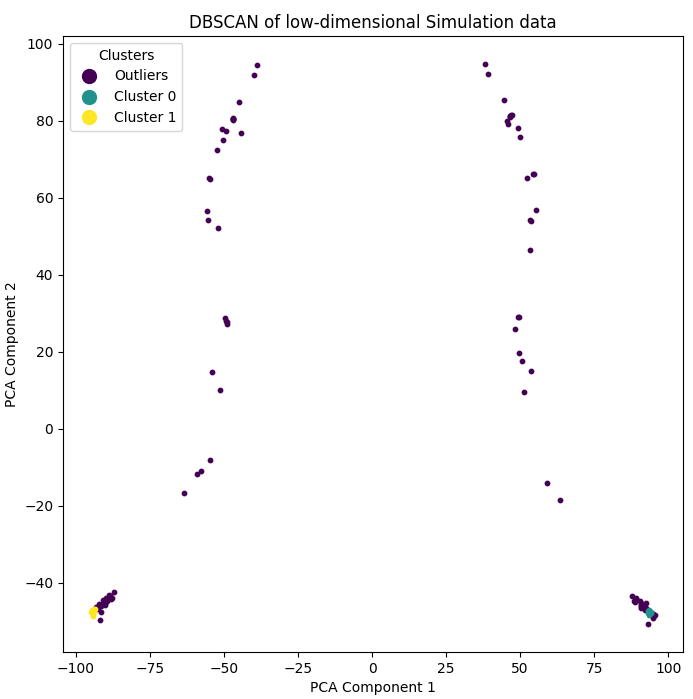
\includegraphics[width=8cm]{images/Clustering/dbscan_pca_sim.png}
    \caption{DBSCAN clustering visualized on PCA-reduced steady-state simulation data.}
    \label{dbscanpca}
    \end{figure}
\begin{figure}[ht]
\centering
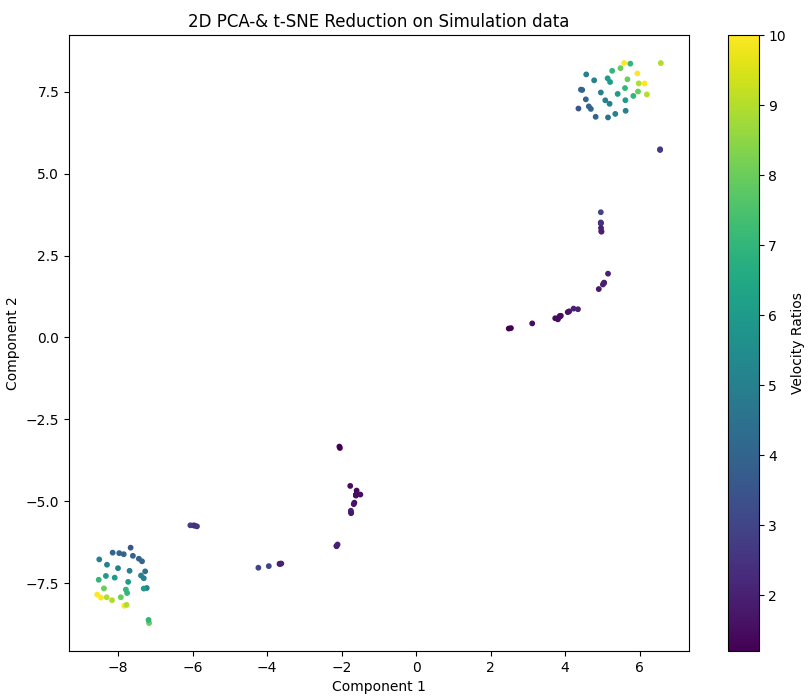
\includegraphics[width=10cm]{images/Clustering/pca_tsne_sim_cmap.png}
\caption{Scatter plot visualizing the subsequent PCA and t-SNE reduction of steady-state simulation data, categorized by varying velocity ratios. }
\label{pcatsnesim}
\end{figure}
\begin{figure}[ht]
    \centering
    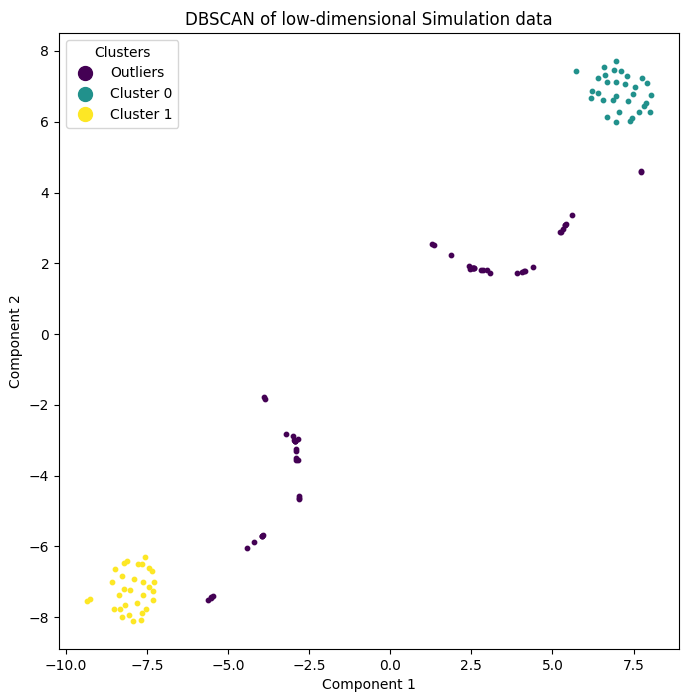
\includegraphics[width=10cm]{images/Clustering/dbscan_tsne_pca_sim.png}
    \caption{DBSCAN clustering visualized on subsequent PCA and t-SNE reduced steady-state simulation data.}
    \label{dbscanpcatsne}
    \end{figure}
% This plot substantiates the ability of the steady-state data, in contrast to the transitional flow data, to manifest clear and structured patterns. Each point on the plot corresponds to a sample from the training-validation dataset. The annotation of case numbers to each point and the above hypothesis about clusters is validated by visual inspection of cases, i.e; if the Coanda adhesion has occurred and the direction of jet deflection. The resultant categorization of the flow behaviors, based on the clustering outcomes, underscores the unsupervised learning techniques' utility in gleaning meaningful insights from complex datasets. \\
Additionally, we reduce the simulation data to a one-dimensional representation, as demonstrated in Figure \ref{1dtsne}. We observe that the data points are distinctly clustered even along the single t-SNE component axis, indicating that the t-SNE algorithm has successfully captured and represented the variance within the high-dimensional dataset in a one-dimensional space. We can also see the emergence of distinct clusters, each cluster denoting a type of fluid behavior. \\
It is to be noted that t-SNE has an element of randomness in the way it projects high-dimensional data into a lower-dimensional space. This randomness is due to the stochastic nature of the algorithm, particularly in the initial placement of points in the low-dimensional space. The orientation and the exact position of the clusters in the map are not fixed and can differ by a rotation or reflection. This is because t-SNE does not preserve the orientation or the exact distances; instead, preserves the local structure of the data and the global relationships between clusters. \\
For the transitional state, t-SNE did not reveal any distinct clusters, indicating that at this early stage, the flow behaviors do not exhibit clear patterns that can be distinguished. 
\begin{figure}[ht]
    \centering
    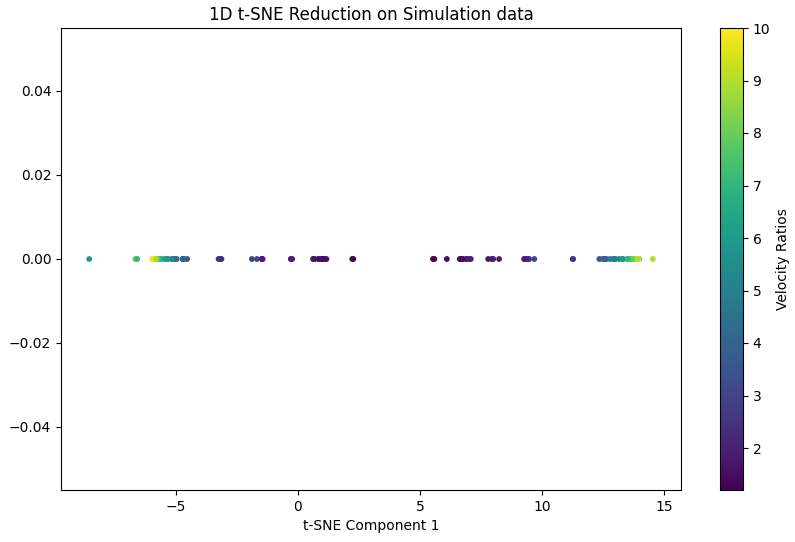
\includegraphics[width=10cm]{images/Clustering/tsne_sim_1dcmap.png}
    \caption{Visualization of 1D t-SNE-reduced steady-state simulation data}
    \label{1dtsne}
    \end{figure}


% \subsection{GNN Encoder}
% The encoder segment of a GNN architecture learns a condensed, low-dimensional representation of the graph-based simulation data, facilitating subsequent analysis. Given a graph $G$ with nodes and edges representing complex relationships, the GNN encoder aims to capture the essential information in a lower-dimensional space, referred to as the latent space representation $Z$, which can be expressed as $Z = \text{Encoder}(G)$. This process not only simplifies the data but also retains significant structural and feature-related information crucial for understanding the underlying patterns of the graph.